\section{Current Error Amplifier}

\begin{figure}[H]
\centering
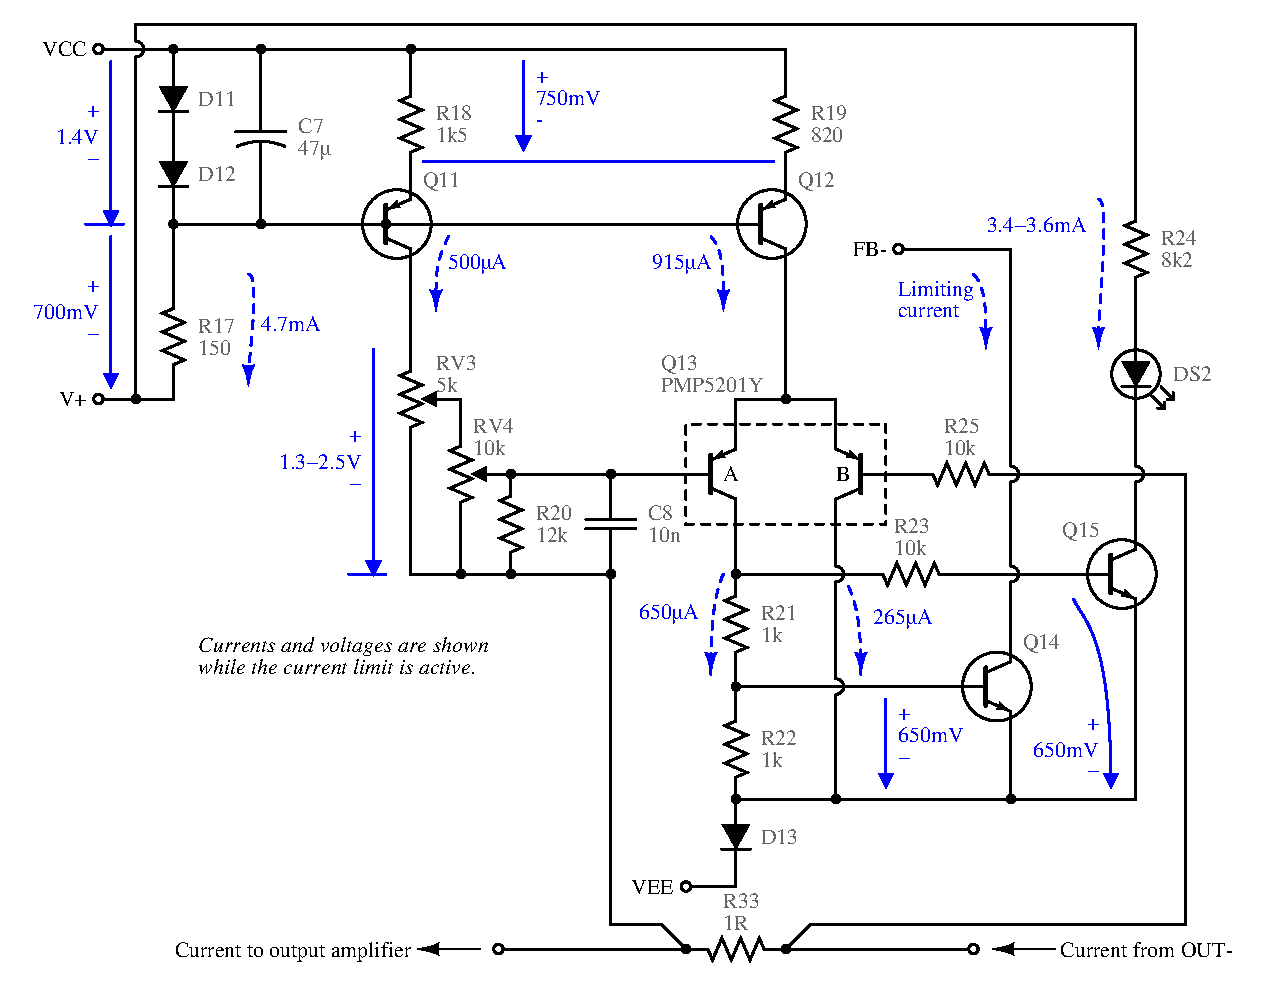
\includegraphics[width=5.5in]{sch/ierror}
\caption{Current error amplifier sub-schematic}
\label{fig:ierror}
\end{figure}

\begin{multicols}{2}

The current error amplifier is similar. The output current $I$ passes through a
1~$\Omega$ resistor, \texttt{R33}, which causes a drop by Ohm's law of $V =
I(1\;\Omega)$. (Note that because the sense lines connect on the output side
of \texttt{R33}, they cancel this drop at the output.) Another long-tailed pair
compares this drop to a reference level.

\subsubsection{Reference}
\texttt{D11} and \texttt{D12} establish a 1.4\;V reference voltage, in the same
way as \texttt{D4}, \texttt{D5} and \texttt{D6} (Fig. \ref{fig:localreg}). The
reason two separate diodes are used, rather than simply using the voltage
between \texttt{D4} and \texttt{D5}, is that the output current itself passes
through \texttt{D4} and \texttt{D5}. This would be a source of error, causing
the current limit to increase as the output current increased. This positive
feedback could lead to oscillation, and would certainly at least lead to an
incorrect limit level.

\subsubsection{Biasing and Potentiometer}
This reference controls two current sources, \texttt{Q11} and \texttt{Q12}, in
the same way as \texttt{Q7} in the voltage error amplifier (Fig.
\ref{fig:verror}). The current through \texttt{Q11} feeds into \texttt{RV3},
which then goes to the inner side of \texttt{R33}. Because the current is
constant, \texttt{RV3} experiences a constant Ohmic voltage drop, and the
bottom end of \texttt{RV3} is fixed at the same voltage as the inner side
of \texttt{R33}. \texttt{RV3} is trimmed to set the highest current limit,
and \texttt{RV4} sits on the front panel, allowing the output current limit to
be set. In the same function as \texttt{R6} (Fig. \ref{fig:reference}),
\texttt{R20} ensures that the current limit defaults low if the current control
potentiometer is disconnected or damaged.

\subsubsection{Limiting Action}
When the current reaches the limit value, the voltage on the outer side of
\texttt{R33} will be equal to the voltage at the output of \texttt{RV4}.
The voltage on \texttt{Q13B}'s base will rise towards its emitter, and it will
stop conducting. At the same time, \texttt{Q13A} will begin conducting. The
current through it flows through \texttt{R22}, causing a voltage drop which
activates \texttt{Q14}, pulling down the inverting feedback line and dropping
the output voltage.

The same current flows through \texttt{R21}, causing another voltage drop,
which is applied to \texttt{Q15}'s base. This turns on LED \texttt{DS2},
indicating to the operator that the current limit is active.

\texttt{C8} fulfills a similar purpose to \texttt{C6} in the voltage error
amplifier (Fig. \ref{fig:verror}): compensating for feedback lags to stabilize
the amplifier. At the same time, it fulfills the same purpose as \texttt{C5} in
the voltage reference (Fig. \ref{fig:reference}), shunting away any
electromagnetic interference picked up by the cable to the panel.

\subsubsection{Protection}
\texttt{R25} protects \texttt{Q13B} from a sudden voltage spike if the output
is shorted or a voltage is applied to it. If a voltage greater than 32.4\;V
is applied to the output,
\texttt{Q13B} would be reverse-biased from
OUT- to VEE; \texttt{D13} protects it from this.

\end{multicols}
